\section{3D Deep Learning}

对于点云来说,直接拉成vector显然是不行的.因为点云本身无序.有一些直接的处理方法:转换成voxel grid(从点云到表面,再重建voxel),或者2D 投影(这属于是越活越回去了).我们想要的network需要对$N!$种不同的点云顺序具有不变性.

一种想法:排序赋予序关系如何?

我们用Permutation Invariant的函数:Symmetric Function.也就是
\begin{equation}
    f(x_1, x_2, \cdots, x_n) \equiv f(x_{\pi_1}, x_{\pi_2}, \cdots, x_{\pi_n}), \forall x \in \mathbb R^N
\end{equation}

实际上,这样的函数随处可见.比如均值,极值等.文献\cite{PointNet} 、PointNet.\footnote{王老师:"虽然我不在这个组里,但PointNet这篇论文的诞生我也是亲眼目睹过的,ICCV的投稿截止在11月,9月底大家还不知道投什么,于是有人说要不试试PointNet吧.写到最后只有两个周调参了,还是打不过voxel,于是加了T-transform.我们这里不讲,因为现在几乎没有用这个的了".(笑)}
\begin{figure}[htbp]
    \centering
    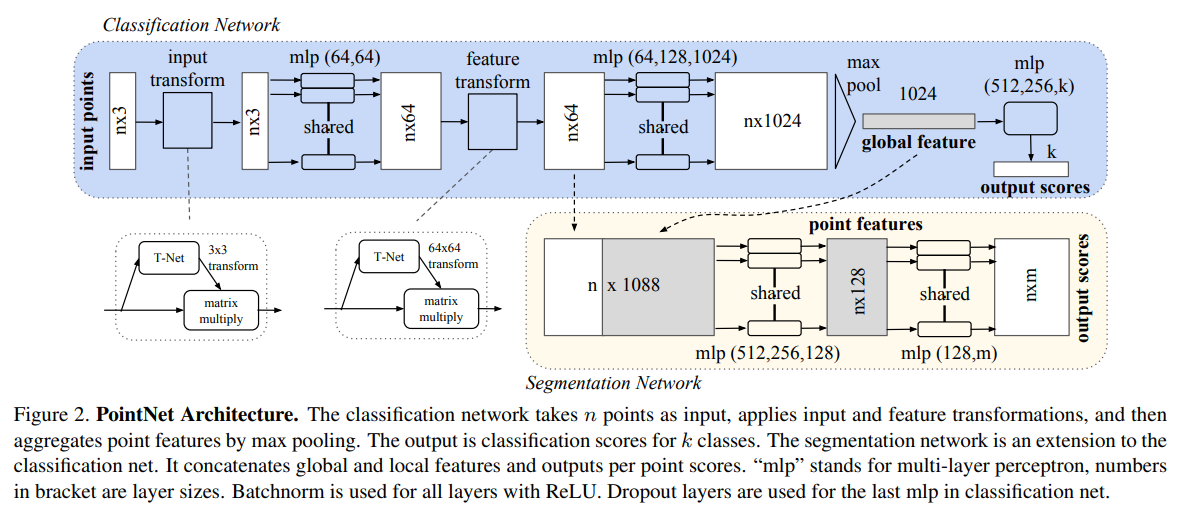
\includegraphics[scale=0.6]{figures/PointNet.png}
    \caption{PointNet的结构图}
    \label{}
\end{figure}

做segmentation:将每个点自身的特征(local)和global feature结合,过MLP就能进行分类.

诸多挑战:Resolution,Occlusion,Noise,Registration.

PointNet对于Resolution和Noise比较robust.在ModelNet40上,去掉50\%的数据,Furthest的准确率只下降了2\%.
能够如此稳定的关键在于max函数,在连续取样时,一些点的丢失可以用周围的点来弥补.而且如果pointnet只有1024个feature,
那么它最多也只会选取1024个点,可能去掉的点根本就没有用到.

PointNet的不足

一步直接maxpooling,没有local context.因此有了PointNet++.它仍是目前不追求过高性能时对point cloud处理的首选方法.
即设定一定的范围,将某个点及其周围的点过MLP,再maxpooling.等同于在image里进行conv.当然,求neighbour可能比较花时间.
另外,所有的neighbour都通过了同样的MLP,毕竟在点云里也无法和图像一样,区分哪个在什么方向.

此外,pointnet++怎么进行分辨率下降呢?2d中是pooling,而pointnet则进行grouping,从前面借.

在恢复的时候,添加的点没有feature,如何处理(2D可以进行Deconv,自然具有特征)?添加interpolate,
新的点选择与它最近的三个点,按照距离反比为权插值获得特征.

3D:voxel Net->sparse conv,屏蔽没有值的voxel,Hash有值的坐标,从NVIDIA,cuda的层次写起.

Sparse conv: kernel 是空间各向异性(spatial anisotropic)的.因此它的acc能够达到惊人的70\%以上,
而point cloud无论如何添加特性,最多也在64\%左右.而且因为可被标签,使用更加方便.但是它的分辨率受限.

Point cloud:高分辨率,鲁棒性,但是表现略差.

\subsection{PointNet++ V.S. Conv}

PointNet++相当于卷积网络的先做 1*1 conv 然后 n*n MaxPooling,都是变少了点的数目,但是每一个点的特征变多了

区别在于:PointNet++对于一个局域部分,不同的点是各向同性的,但是卷积网络对于一个局域是不同的,因为一个卷积核不同位置的权不一样.

具体表现在:如果把一个邻域内的点更换位置,那么PointNet++的结果不变,但是卷积网络的结果会变.

这是由于两个原因:
\begin{enumerate}
    \item 卷积网络的卷积核是 3*3 的,而PointNet++的MLP是全局的,相当于1*1的CONV,而1*1的CONV很容易想到是各向同性的,
    如果把一个邻域内的点更换位置,那么每个点的MLP结果不变.
    \item 卷积网络的MaxPooling不是全局的,而PointNet++的MaxPooling是全局的,因此如果把一个邻域内的点更换位置,
    那么卷积网络的结果会变,而PointNet++的结果不变,因为怎么变换位置都是取最大值.
\end{enumerate}

参数量: $C\times C^\prime$ V.S. $3\times 3\times 3\times C\times C^\prime$

\subsection{设计一个二维PointNet}

如何设计一个二维的pointnet呢?

我们可以将图片看作二维的点云, 对于每一个像素 $x_i$, 将其颜色或者透明度等信息看作是 $x_i$ 的三维坐标,然后使用pointnet的方法进行处理

具体来讲, 图片维度为 $H\times W\times C$, 那么我们可以将其看作 $H\times W$ 个点, 每个点的特征是 $C$ 维的, 
每一个像素通过相同的MLP映射到 $C^\prime$ 维, 然后进行maxpooling, 最终得到 $C^\prime$ 维的全局特征.